\section{ПРОГРАММА И МЕТОДИКА ИСПЫТАНИЙ}
\label{sec:test}
Тестирование разрабатываемых программных продуктов является\break крайне важным процессом. Тестирование позволяет избежать
лишних затрат на разработку, так как ошибки, возникающие в процессе разработки ПО,\break вскрываются как можно раньше. Также
исправление как можно большего количества ошибок перед релизом позволяет избежать затрат на исправление ошибок после
внедрения ПО.

Тестирование позволяет не только выявить ошибки в программном коде, но и вычислить фрагменты кода, требующие
оптимизации. Выполнение этой функции облегчают инструменты трассировки и профилирования кода.

Тестирование программы проводилось на компьютере со следующими характеристиками:
\begin{itemize}
	\item центральный процессор -- Intel Core i5-5200U с тактовой частотой 2.20ГГц;
	\item объем оперативной памяти -- 4 ГБ;
	\item операционные системы: ArchLinux x86\_64, Windows 10 x86\_64\break Education Edition.
\end{itemize}

\subsection{Отладчик GDB}
\label{sec:test:gdb_debug}
В качестве отладчика был выбран GDB, так как он может быть использован для тестирования как и в ОС Linux, так и в ОС
Windows. GDB также позволяет использовать отладчик, используя графический интерфейс. Для этого можно использовать
подключение GDB в качестве инструмента отладки к многим популярным IDE.

Для запуска отладчика необходимо наличие в отлаживаемой программе таблицы символов. Для этого требуется компиляция
проекта в debug режиме. В release версии таблица символов удаляется для экономии места и затруднения эксплуатации
возможных уязвимостей.
\begin{figure}[htb]
	\centering
	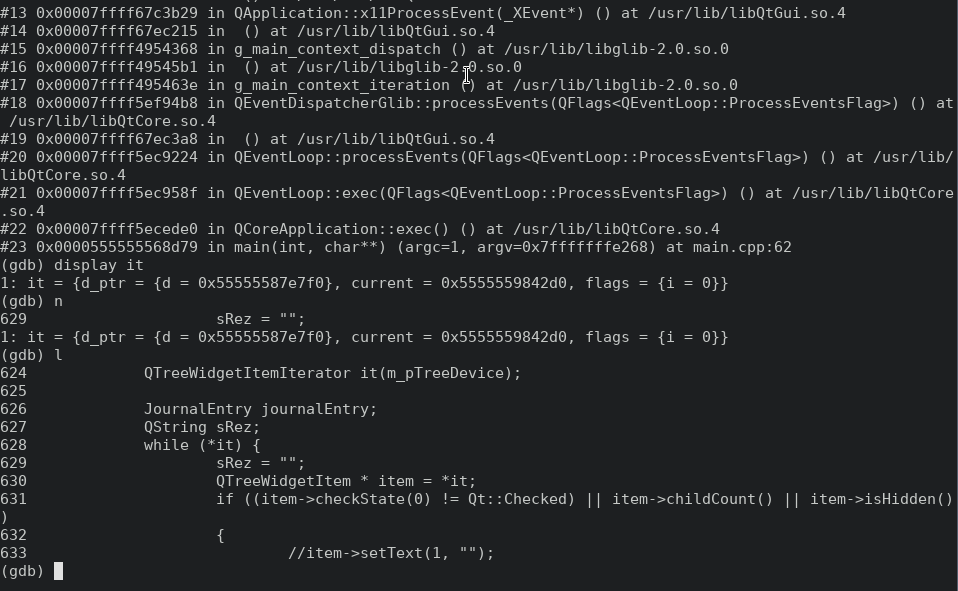
\includegraphics[scale=0.6]{gdb}
	\caption{Работа с gdb через консоль}
	\label{fig:test:gdb_debug:gdb}
\end{figure}

В процессе отладки большинство ошибок было устранено при использовании gdb через консоль. Пример окна отладки
представлен на рис. \ref{fig:test:gdb_debug:gdb}. При отладке пригодились следующие возможности gdb:
\begin{itemize}
	\item просмотр кода отлаживаемой функции;
	\item механизм контрольных точек;
	\item просмотр состояния переменных во время исполнения;
	\item постоянное отображения выбранных переменных с помощью команды \texttt{display};
	\item вывод стека вызова функций;
	\item изменение содержимого переменных в ходе отладки;
	\item анализ причины внезапного закрытия приложения с помощью анализа core файлов.
\end{itemize}

С помощью gdb удалось выявить ряд ошибок, которые были связаны с доступом за пределы выделенной памяти, использованием
данных через указатель после освобождения памяти, формированием неправильных выходных данных алгоритмами.

\subsection{Использование Valgrind для отладки использования памяти}
\label{sec:test:valgrind}
В ходе разработки и отладки дипломного проекта были выявлены проблемы связанные с утечкой памяти, повторным
использованием памяти, использованием неинициализированнной памяти, использованием памяти, которая находится за
пределами выделенного блока. Для решения этих и других проблем, после анализа существующих инструментов отладки и
профилирования, было принято решение использовать пакет Valgrind, который распространяется под лицензией GPL.

Valgrind представляет собой виртуальную машину, на которой происходит исполнение программы и ее анализ с помощью
различных инструментов, входящих в пакет Valgrind. Данная виртуальная машина использует метод динамической
перекомпиляции для запуска программы. Valgrind транслирует программу в промежуточное представление, после преобразования
для отладки программы могу быть использованы инструменты, входящие в Valgrind, данные инструменты проводят необходимые
преобразования программы, находящейся в промежуточном представлении, после чего происходит трансляция программы в
машинный код.

Преобразования значительно замедляет работу программы. Разработанная программа не содержит алгоритмов, требующих больших
затрат ресурсов вычислительной системы, поэтому использование инструментов, входящих в пакет Valgrind, является
целесообразным.

Пакет Valgrind содержит в себе набор инструментов для отладки и профилирования программы. В ходе разработки и отладки
проекта были использован инструмент Memcheck. Далее будет приведен краткий обзор этого инструмента.
\begin{figure}[htb]
	\centering
	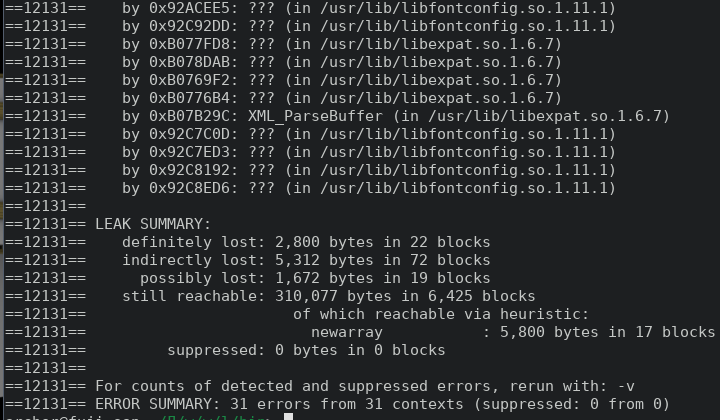
\includegraphics[scale=0.8]{memcheck}
	\caption{Результаты анализа программы с помощью Memcheck}
	\label{fig:test:valgrind:memcheck}
\end{figure}

Инструмент Memcheck (рис. \ref{fig:test:valgrind:memcheck}) используется для анализа ошибок, связанных с некорректной работой с памятью. Данный инструмент
используется по умолчанию в пакете Valgrind. Memcheck вставляет дополнительный код вокруг инструкций, которые
производят выделение памяти, также производит маркировку памяти. Memcheck помечает участки памяти, находящиеся за
границами выделенных блоков как некорректные, что позволяет детектировать ошибки, связанные с выходом за пределы
выделенной области памяти. Memcheck помечает блоки памяти флагами валидности (определяет, была ли память
проинициализированна) и адресуемости (определяет, относится ли данный участок памяти к выделенному блоку). Изменение состояния маркеров в ходе выполнения программы и
анализ данных маркеров позволяют выполнять обнаружение следующих ошибок при работе с памятью:
\begin{itemize}
	\item утечка памяти;
	\item доступ к памяти за пределами выделенного блока;
	\item доступ к памяти после ее освобождения;
	\item использование неинициализированнной памяти.
\end{itemize}

\subsection{Использование программ-имитаторов}
Работа разработанной системы функционального контроля\break технических средству КМУ артиллерийского дивизиона тесно связана с
взаимодействием с различным оборудованием. Многие из технических средств имеют большие габариты, требуют подключения
через интерфейс RS-232 либо получение данных от них требует значительных временных затрат. Тестировать работу программы
с реальным оборудованием в \company~возможно либо в специальном помещении, выполняющем роль тестового полигона, либо
непосредственно на боевой машине. Рассмотрим недостатки и преимущества каждого из данных подходов.

Тестовый полигон представляет собой помещение с десятью компьютерами, к каждому из которых подключена различная
периферия, используемая в армейских подразделениях. Данный кабинет удобно использовать в первую очередь проектным командам для
совместного тестирования работы программ на реальном оборудовании, обсуждения проблем, возникающих при работе с
оборудованием, и рассмотрения новых путей их решения. Недостатком работы на тестовом полигоне является сложность
подключения большого количества устройств к компьютеру для проведения тестирования работы системы. Другими недостатками
являются: невозможность постоянной работы на полигоне, ввиду использования полигона несколькими командами, сложность
коммуникации с коллегами, ввиду нахождения полигона вдалеке от помещений разработчиков.

Тестирование работы программы на боевой машине позволяет проверить работу программы непосредственно в месте, где она
будет впоследствии развернута. Данный подход актуален на финальных стадиях разработки системы, когда необходимо
проверить нюансы работы в среде, близкой к условиям эксплуатации. В процессе тестирования в данной системе возможно
обнаружить сложнодетектеруемые в других условиях ошибки, такие как проблемы взаимодействия компьютеров в локальной сети
машины, либо проблемы в работе некоторых устройств тестовой среды. Данная среда не предназначена для разработки
программ, так как в машинах отсутствует связь с сетью Интернет, техника доступна лишь на небольшое количество времени и
может находиться вдали от офиса разработки.

Для повышения производительности труда и абстрагирования от работы реальных физических устройств в компании \company~были
разработаны специальные программы-имитаторы. Данные программы позволяют создавать виртуальные устройства, работающие по
необходимо протоколу. Подключение программ-имитаторов к системе осуществляется либо через виртуальные последовательные
порты, либо через сокетное соединение. Программы-имитаторы принимают сообщения от разрабатываемых программных модулей и
автоматически формируют соответствующие ответные сообщения. Также разработчик может настроить параметры устройства и
сформировать желаемую команду через графический интерфейс программы-имитатора (рис.\ref{fig:test:imitators:imitator}).
\begin{figure}[htb]
	\centering
	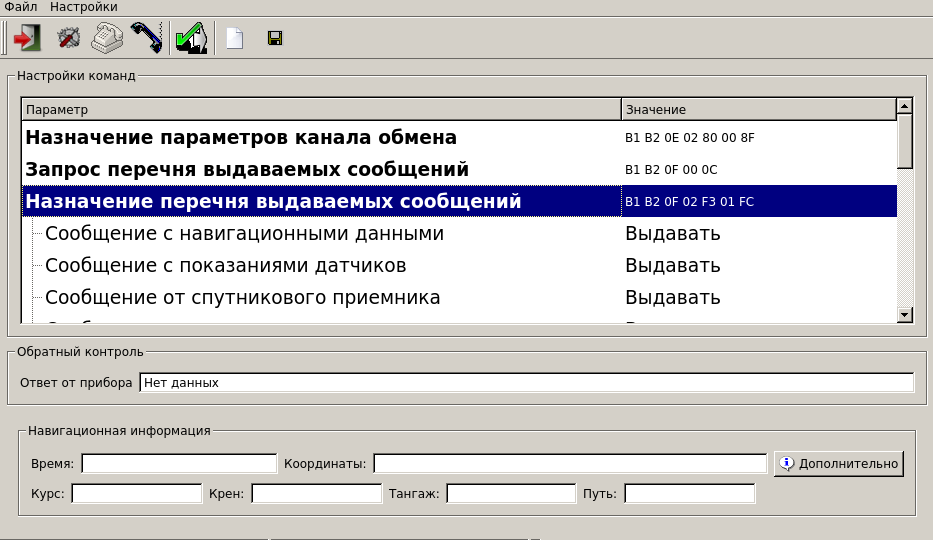
\includegraphics[scale=0.65]{imitator}
	\caption{Имитатор устройства, использующего протокол БИНС-3}
	\label{fig:test:imitators:imitator}
\end{figure}
